
\subsection{Case 1: Primary Frequency Control}
For example, for primary frequency control, which expects a step response from a nominal set-point to a new set-point based upon the frequency deviation, the TSO needs to establish two parameters:
\begin{itemize}
\item Optimal ramp time per bid atom
\item Optimal service duration
\end{itemize}

The optimal ramp time needs to be defined by the TSO, and will be derived from the inertia of the system. For example, the Danish TSO could determine that the optimal ramp time to be 0.001 s.

The optimal service duration depends solely on how fast it is able to activate secondary reserves. Again, in the Danish case 15 minutes is chosen to be the optimum.

Thus the performance value of units expecting to provide primary frequency control services can be characterised by:
\begin{align}
\kappa &= \alpha_1 \frac{\tau_{r,0}}{\max({\tau_{r,0},\tau_{r,a})}} + \alpha_2  \frac{\min(\tau_0,\tau_{a})}{\tau_{0}}\label{eq:kappa_primfreq}\\
\sum_{i} \alpha_i &= 1
\end{align}
where $\tau_{r,a}$ is the actual ramping time that the AS-providers can deliver, $\tau_{r,0}$ is the optimal ramping rate that the TSO would like to have. Similarly, $\tau_a$ is the endurance time that providers can deliver, and $\tau_{0}$ the the ideal endurance time the TSO would like. 
The TSO can assign a priority to any of the two variables by adjusting the weight factor $\alpha \in [0,1]$.

The formulation of equation~\eqref{eq:kappa_primfreq} has the property that a fast responding/short endurance service provider may be as valuable as a slow responding/long endurance service provider. 

\subsection{Case 2: Load Frequency Control}

E.g. for AGC/regulation/LFC:

1) The system requirements for the AS are: 
\kh{Esteban, what's the numbers again? cheers}
\begin{itemize}
\item Maximum ramp time for procurement volume $\tau_r$
\item Maximum activation time for 5\% procurement volume $\tau_{r5}$
\item Expected (minimum) duration of service $\tau_E$
\end{itemize}

2) \textbf{Tender:}
$P_{R,tot}$ total volume

Bid Parameters: 
$P_{R,a}$ - bid volume, $R_{a}$ - ramp rate, $\tau_a$ - duration 
\kh{i am not sure if we should formulate the limit as 'energy' or as 'duration', as the effects are quite different in case of partial activation --kai}


Other Service properties:

Performance parameter:
\begin{align}
\kappa &= \alpha_1 \frac{\min({R_{0},R_a})}{R_0} + \alpha_2  \frac{\min(\tau_0,\tau_{a})}{\tau_{0}}\label{eq:kappa2}\\
\sum_i\alpha_i &=1
\end{align}

3) 

\begin{figure}[htb!]
\centering
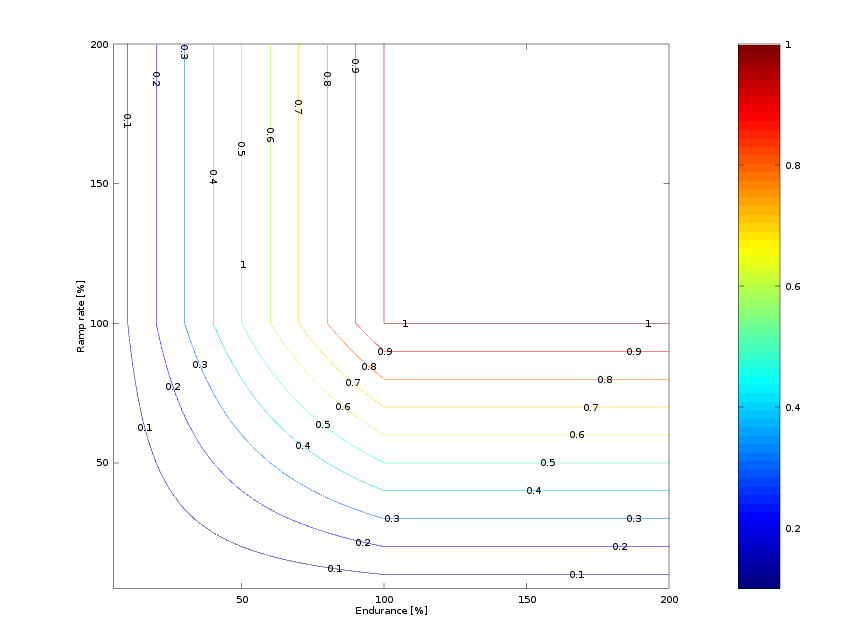
\includegraphics[width=1\columnwidth]{utility_ramp_endurance.png}
\caption{Caption it yourself!}
\label{fig:utrend}
\end{figure}